\input{header.tex}

\setcounter{theorem}{22}
\begin{exercise}[BH.2.23] 
	\begin{solution}
	It's easiest to make a drawing. Let blue denote the event $G$.
	\begin{center}
		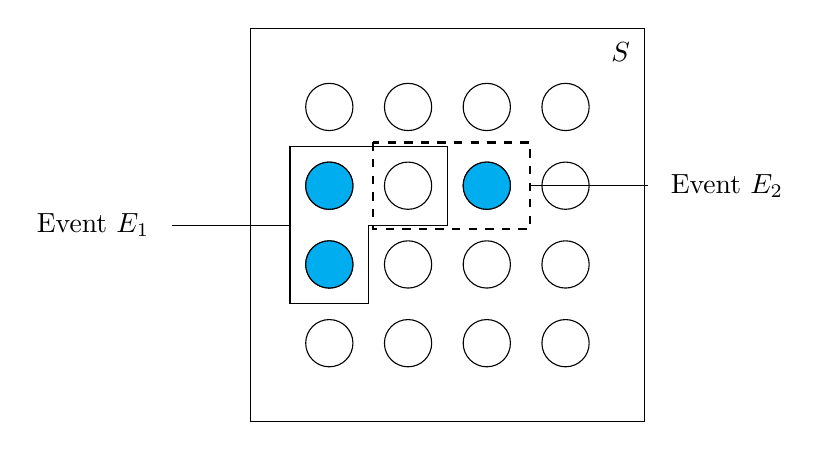
\begin{tikzpicture}
			\draw (0,0) -- (5,0) -- (5,5) -- (0,5) -- (0,0);
			\node at (4.7,4.7) {$S$};
			\foreach \x in {1,...,4} 
			\foreach \y in {1,...,4}
			{\draw (\x,\y) circle (0.3cm);}
			\draw[fill=cyan] (1,2) circle (0.3cm);
			\draw[fill=cyan] (1,3) circle (0.3cm);
			\draw[fill=cyan] (3,3) circle (0.3cm);
			\draw (0.5,3.5) -- (0.5,1.5) -- (1.5,1.5) -- (1.5,2.5) -- (2.5,2.5) -- (2.5,3.5) -- (0.5,3.5);	
			\draw (-1,2.5) -- (0.5,2.5);
			\node at (-2,2.5) {Event $E_{1}$}; 
			\draw[dashed,thick] (1.55,3.55) -- (1.55,2.45) -- (3.55,2.45) -- (3.55,3.55) -- (1.55,3.55);	
			\draw (3.55,3) -- (5.05,3);
			\node at (6.05,3) {Event $E_{2}$}; 
		\end{tikzpicture}
	\end{center}
	We see that $P(G) = 3/16$, $P(G|E_{1})=2/3$, $P(G|E_{2})=1/2$, yet $P(G|E_{1},E_{2})=0$. E.g., $E_i$ denote that person is robbed by someone (if you feel like the only one carrying out a crime, the guilty level might be high, but unfortunately the guilty may reduce when you learn someone else also robbed,  Broken windows theory.)
\end{solution}
\end{exercise}
\input{trailer.tex}
